\section{Least Squares Approximation}
Consider the following setup with $n > p$:
\begin{itemize}
    \item $X \in \mathbb{R}^{n \times p}$: feature matrix with $n$ samples and $p$ features, where $\text{rank}(X) = p$
    \item $\underline{y} \in \mathbb{R}^n$: label vector for each sample
\end{itemize}
The feature matrix $X$ can be written as:
\[
X = 
\begin{bmatrix}
    \horzbar & \underline{x_1^\intercal} & \horzbar\\
    \horzbar & \underline{x_2^\intercal} & \horzbar\\    
     & \vdots & \\
    \horzbar & \underline{x_n^\intercal} & \horzbar
\end{bmatrix}
\]
where $\underline{x_j}$ is the $j$-th column of $X$.

Given a new sample $\tilde{\underline{x}}$, we aim to predict its corresponding label $\tilde{y}$ using the information from the training set. We can use a linear model:
\[
    \tilde{y} = \tilde{\underline{x}}^\intercal \underline{w}, \quad \underline{w} \in \mathbb{R}^p
\]

Since $\underline{y} \neq X\underline{w}$ in general, we use the approximation $\hat{\underline{y}} = X\underline{w}$. Thus, $\hat{\underline{y}} \in \mathcal{C}(X)$, while $\underline{y} \notin \mathcal{C}(X)$ in general.

The prediction error for the $i$-th sample is given by:
\[
    r_i(\underline{w}) = \underline{y_i} - \underline{\hat{y_i}}    
\]
The goal is to minimize the squared $\ell_2$-norm of the residual vector $\underline{r}(\underline{w})$:
\[
    \hat{\underline{w}} = \underset{\underline{w}}{\arg\min}\,||\underline{r}(\underline{w})||^2_2
\]
There are two approaches to solve this problem:
\begin{enumerate}
    \item Geometrical interpretation
    \item Optimization procedures
\end{enumerate}

\subsection*{Geometrical Interpretation}
\begin{center} 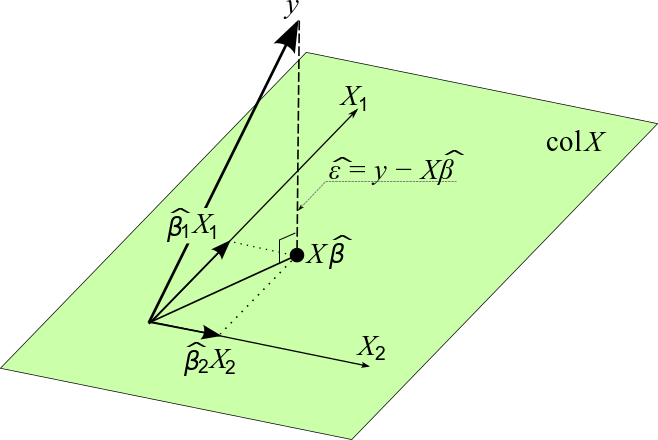
\includegraphics[scale = 0.4]{../images/OLS_geometric_interpretation.png} \end{center}
\begin{itemize}
    \item The plane represents the space of predictions $\mathcal{C}(X)$, spanned by the column vectors of $X$.
    \item $\underline{y}$ is the label vector to be predicted.
    \item $\hat{\underline{y}} = X\hat{\beta}$ is the projection of $\underline{y}$ onto $\mathcal{C}(X)$.
    \item $\underline{r}(\underline{w}) = \epsilon$ is the residual vector, representing the error between the predicted and actual labels.
\end{itemize}
For any $\underline{\overline{y}} \in \mathcal{C}(X)$ different from $\hat{\underline{y}}$, with residuals $\underline{\overline{r}} = \underline{y} - \underline{\overline{y}}$ and $\underline{\hat{r}} = \underline{y} - \underline{\hat{y}}$, we have:
\[
    ||\underline{\hat{r}}||_2 \leq ||\underline{\overline{r}}||_2
\]
This is because $\underline{\hat{r}}$ is the orthogonal projection of $\underline{y}$ onto $\mathcal{C}(X)$, and the orthogonal projection is the closest point to $\underline{y}$ in the subspace $\mathcal{C}(X)$.

Consequently, we have:
\[
    \underline{x_j^\intercal}\underline{\hat{r}} = 0, \quad j = 1, \dots, p    
\]
The residual vector $\underline{\hat{r}}$ is orthogonal to each column vector of the feature matrix $X$, meaning it is perpendicular to the subspace spanned by the columns of $X$.
In matrix form:
\[
    X^\intercal \underline{\hat{r}} = \underline{0} \implies X^\intercal (\underline{y} - \underline{\hat{y}}) = \underline{0} \implies X^\intercal (\underline{y} - X\underline{\hat{w}}) = \underline{0} \implies X^\intercal \underline{y} = X^\intercal X \underline{\hat{w}}
\]
If $X$ is full rank, then $X^\intercal X$ is also full rank and invertible. Thus, we can find $\hat{\underline{w}}$ as:
\[
    \hat{\underline{w}} = (X^\intercal X)^{-1}X^\intercal \underline{y}
\]


\subsection*{Optimization Perspective}
We can solve the problem using optimization techniques:
\[
    \hat{\underline{w}} = \underset{\underline{w}}{\arg\min}||\underline{r}(\underline{w})||^2_2 = \underset{\underline{w}}{\arg\min}||\underline{y} - X\underline{w}||^2_2 = \underset{\underline{w}}{\arg\min}(\underline{y} - X\underline{w})^\intercal(\underline{y} - X\underline{w})
\]
\[
    = \underset{\underline{w}}{\arg\min} \bigg[\underline{y}^\intercal \underline{y} - 2\underline{y}^\intercal X\underline{w} + \underline{w}^\intercal X^\intercal X\underline{w}\bigg] = \underset{\underline{w}}{\arg\min} F(\underline{w})
\]
$F(\underline{w})$ is a quadratic functional. If $X$ is full rank, then $X^\intercal X$ is positive definite, implying that the functional is strictly convex and has a unique minimum.

Setting the gradient to zero:
\[
    \nabla_{\underline{w}}F(\underline{w}) = -2X^\intercal \underline{y} + 2X^\intercal X\underline{w} = \underline{0}
\]
leads to the same solution as the geometrical interpretation.


We have obtained:
\[
    \underline{\hat{w}} = (X^\intercal X)^{-1} X^\intercal \underline{y} \implies \underline{\hat{y}} = \underbrace{X(X^\intercal X)^{-1} X^\intercal}_{P_x} \underline{y}     
\]
The matrix $P_x$ dimension is given by the product of: $(n\times p)(p\times p)(p \times n) = (n\times n)$ and has this properties:
\begin{itemize}
    \item $P_x = P_x^2$
    \item $P_x$ is a projection matrix
\end{itemize}

Let's consider $U$ an orthogonal ($U^\intercal U = I$) matrix that contains the basis for $\mathcal{C}(X)$ this means that $\mathcal{C}(X) = \mathcal{C}(U)$. We can write:
\[
    \underline{\hat{y}} = X\underline{\hat{w}} = U\underline{\tilde{w}}    
\]
So this basically means that the predicted value of $y$ still a projection on a plane but this time the plane is spanned by the columns of $U$ and not by the columns of $X$. By substituting last equation in the minimization method for least squares we have:
\[
    \underline{\tilde{w}} = \underset{\underline{w}}{\arg\min} ||\underline{y} - U\underline{w}||^2_2 \implies \underline{\hat{y}} = U\underline{\tilde{w}} = U(U^\intercal U)^{-1}U^\intercal \underline{y} = UU^\intercal \underline{y} 
\]
This formulation is possible because this time in the parenthesis we have an orthogonal matrix and this means that $(U^\intercal U)^{-1} = U^\intercal U = I$. In general $UU^\intercal \neq I$ because it might be rectangular (while $U^\intercal U$ is always square).\\







\subsection*{Ridge regression }
This method will help us in preventing the problem mentioned just before. We start from the definition of the weight vector for linear model explicited for the optimization method of the Least Squares:
\[
    \underline{\hat{w}}_{LS} = \arg \min_{\underline{w}} \underbrace{||\underline{y} - X\underline{w}||_2^2 + \lambda ||\underline{w}||_2^2}_{f(\underline{w})}
\]
In particular we have added a term. 
\[
    f(\underline{w}) = \underline{y}^\intercal \underline{y} - 2\underline{w}^\intercal X \underline{y} + \underline{w}^\intercal X^\intercal X \underline{w} + \lambda \underline{w}^\intercal \underline{w}
\]
We can now compute the gradient of this function:
\[
        \nabla_w(f(\underline{w})) = -2X^\intercal \underline{y} + 2X^\intercal X \underline{w} + 2\lambda \underline{w} = 0      
\]
\[
    X^\intercal \underline{y} = (X^\intercal X + \lambda I)\underline{w}     
\]
\[
    \underline{\hat{w}}_{R} = (X^\intercal X + \lambda I)^{-1} X^\intercal \underline{y}    
\]
It's easy to notice that if $\lambda = 0$ we get the Least Squares solution. If $\lambda > 0$ we will have a different solution. We can now compute the SVD of $X$:
\[
    \begin{split}
        \underline{\hat{w}}_R &= (V\Sigma^\intercal \underbrace{U^\intercal U}_{I} \Sigma V^\intercal + \lambda \underbrace{V V^\intercal}_{I})^{-1} V\Sigma^\intercal U^\intercal \underline{y} \\
        &= \left[V(\Sigma^\intercal \Sigma + \lambda I)V^\intercal\right]^{-1} V\Sigma^\intercal U^\intercal \underline{y} \\
        &= V\underbrace{(\Sigma^\intercal \Sigma + \lambda I) ^{-1}\Sigma^\intercal}_{M}U^\intercal \underline{y} \\
    \end{split}    
\]
Where 
\[
M = \begin{bmatrix}
    \dfrac{\sigma_1}{\sigma_1^2 + \lambda} & 0 & \dots & 0 & 0 & \dots & 0\\
    0 & \dfrac{\sigma_2}{\sigma_2^2 + \lambda} & \dots & 0 & 0 & \dots & 0\\
    \vdots & \vdots & \ddots & \vdots & \vdots & \ddots & \vdots\\
    0 & 0 & \dots & \dfrac{\sigma_p}{\sigma_p^2 + \lambda} & 0 & \dots & 0
\end{bmatrix}
\]
\begin{itemize}
    \item if $\sigma_i$ is big compared to $\lambda$ then $\dfrac{\sigma_i}{\sigma_i^2 + \lambda} \approx \dfrac{1}{\sigma_i}$
    \item if $\sigma_i$ is close to 0 then $\dfrac{\sigma_i}{\sigma_i^2 + \lambda} \approx 0$
\end{itemize}
Ridge regression addresses the problem of singular values close to zero in the matrix $X$ by adding a regularization term $\lambda$ to the diagonal of $X^\intercal X$. This modifies the singular values in the pseudo-inverse term to $\frac{\sigma_i}{\sigma_i^2 + \lambda}$. When $\sigma_i$ is much larger than $\lambda$, the solution remains similar to the Least Squares solution. However, when $\sigma_i$ is close to zero, the corresponding term in the pseudo-inverse becomes approximately zero, mitigating the issues caused by small singular values. As $\lambda$ approaches zero, the Ridge regression solution converges to the Least Squares solution. The choice of $\lambda$ depends on the desired balance between fitting the training data and regularizing the model, and is often selected using techniques like cross-validation.
If $\lambda$ is very small the matrix of $\Sigma$'s is almost equal to $\Sigma^+$.
\[
    \begin{split}
        \underline{\hat{w}}_R &= (X^\intercal X + \lambda I)^{-1} X^\intercal \underline{y}\\
        &= (X^\intercal X + \lambda I)^{-1} X^\intercal(X\underline{w}^* + \underline{\epsilon})\\
        &= (X^\intercal X + \lambda I)^{-1} X^\intercal X\underline{w}^* + (X^\intercal X + \lambda I)^{-1} X^\intercal \underline{\epsilon}\\
    \end{split}    
\]
